\begin{frame}[fragile]{Visualização de uma atualização em uma BITree}

    \begin{figure}
        \centering

        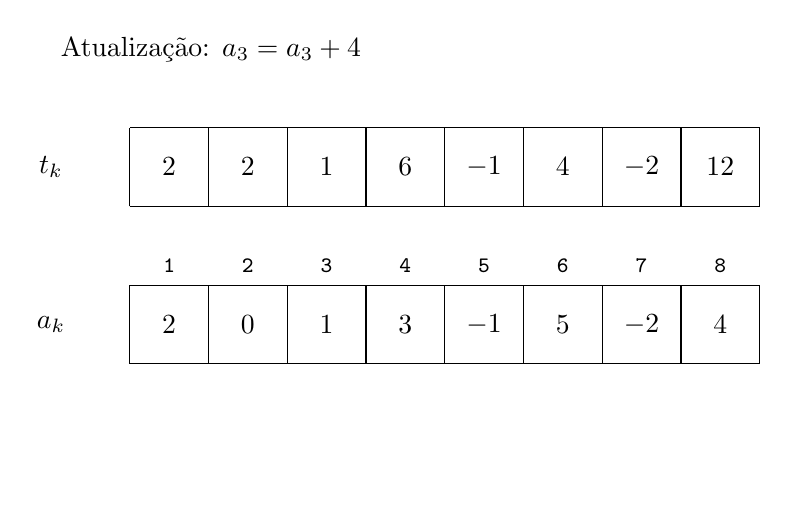
\begin{tikzpicture}
            \node[anchor=west] at (0, 12) { Atualização: $a_3 = a_3 + 4$ };

            \draw (1, 10) grid (9, 11);
            \draw (1, 8) grid (9, 9);

            \node at (0, 8.5) { $a_k$ };
            \node at (0, 10.5) { $t_k$ };

            \node[opacity=0, anchor=west] at (0, 6.5) { $r_1 = 3$ };

            \node at (1.5, 9.25) { \footnotesize \tt 1 };
            \node at (2.5, 9.25) { \footnotesize \tt 2 };
            \node at (3.5, 9.25) { \footnotesize \tt 3 };
            \node at (4.5, 9.25) { \footnotesize \tt 4 };
            \node at (5.5, 9.25) { \footnotesize \tt 5 };
            \node at (6.5, 9.25) { \footnotesize \tt 6 };
            \node at (7.5, 9.25) { \footnotesize \tt 7 };
            \node at (8.5, 9.25) { \footnotesize \tt 8 };

            \node at (1.5, 8.5) { \textcolor{black}{$2$} };
            \node at (2.5, 8.5) { \textcolor{black}{$0$} };
            \node at (3.5, 8.5) { \textcolor{black}{$1$} };
            \node at (4.5, 8.5) { \textcolor{black}{$3$} };
            \node at (5.5, 8.5) { \textcolor{black}{$-1$} };
            \node at (6.5, 8.5) { \textcolor{black}{$5$} };
            \node at (7.5, 8.5) { \textcolor{black}{$-2$} };
            \node at (8.5, 8.5) { \textcolor{black}{$4$} };

            \node at (1.5, 10.5) { \textcolor{black}{$2$} };
            \node at (2.5, 10.5) { \textcolor{black}{$2$} };
            \node at (3.5, 10.5) { \textcolor{black}{$1$} };
            \node at (4.5, 10.5) { \textcolor{black}{$6$} };
            \node at (5.5, 10.5) { \textcolor{black}{$-1$} };
            \node at (6.5, 10.5) { \textcolor{black}{$4$} };
            \node at (7.5, 10.5) { \textcolor{black}{$-2$} };
            \node at (8.5, 10.5) { \textcolor{black}{$12$} };

        \end{tikzpicture}

    \end{figure}

\end{frame}

\begin{frame}[fragile]{Visualização de uma atualização em uma BITree}

    \begin{figure}
        \centering

        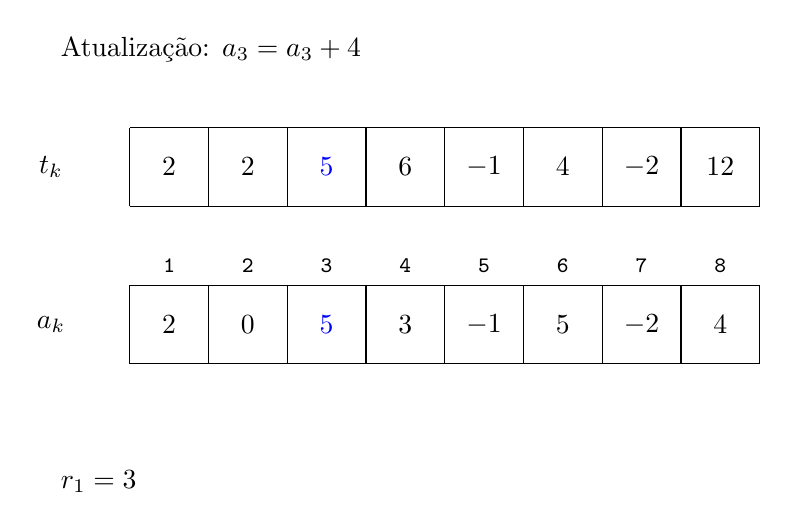
\begin{tikzpicture}
            \node[anchor=west] at (0, 12) { Atualização: $a_3 = a_3 + 4$ };

            \draw (1, 10) grid (9, 11);
            \draw (1, 8) grid (9, 9);

            \node at (0, 8.5) { $a_k$ };
            \node at (0, 10.5) { $t_k$ };

            \node[anchor=west] at (0, 6.5) { $r_1 = 3$ };

            \node at (1.5, 9.25) { \footnotesize \tt 1 };
            \node at (2.5, 9.25) { \footnotesize \tt 2 };
            \node at (3.5, 9.25) { \footnotesize \tt 3 };
            \node at (4.5, 9.25) { \footnotesize \tt 4 };
            \node at (5.5, 9.25) { \footnotesize \tt 5 };
            \node at (6.5, 9.25) { \footnotesize \tt 6 };
            \node at (7.5, 9.25) { \footnotesize \tt 7 };
            \node at (8.5, 9.25) { \footnotesize \tt 8 };

            \node at (1.5, 8.5) { \textcolor{black}{$2$} };
            \node at (2.5, 8.5) { \textcolor{black}{$0$} };
            \node at (3.5, 8.5) { \textcolor{blue}{$5$} };
            \node at (4.5, 8.5) { \textcolor{black}{$3$} };
            \node at (5.5, 8.5) { \textcolor{black}{$-1$} };
            \node at (6.5, 8.5) { \textcolor{black}{$5$} };
            \node at (7.5, 8.5) { \textcolor{black}{$-2$} };
            \node at (8.5, 8.5) { \textcolor{black}{$4$} };

            \node at (1.5, 10.5) { \textcolor{black}{$2$} };
            \node at (2.5, 10.5) { \textcolor{black}{$2$} };
            \node at (3.5, 10.5) { \textcolor{blue}{$5$} };
            \node at (4.5, 10.5) { \textcolor{black}{$6$} };
            \node at (5.5, 10.5) { \textcolor{black}{$-1$} };
            \node at (6.5, 10.5) { \textcolor{black}{$4$} };
            \node at (7.5, 10.5) { \textcolor{black}{$-2$} };
            \node at (8.5, 10.5) { \textcolor{black}{$12$} };

        \end{tikzpicture}

    \end{figure}

\end{frame}

\begin{frame}[fragile]{Visualização de uma atualização em uma BITree}

    \begin{figure}
        \centering

        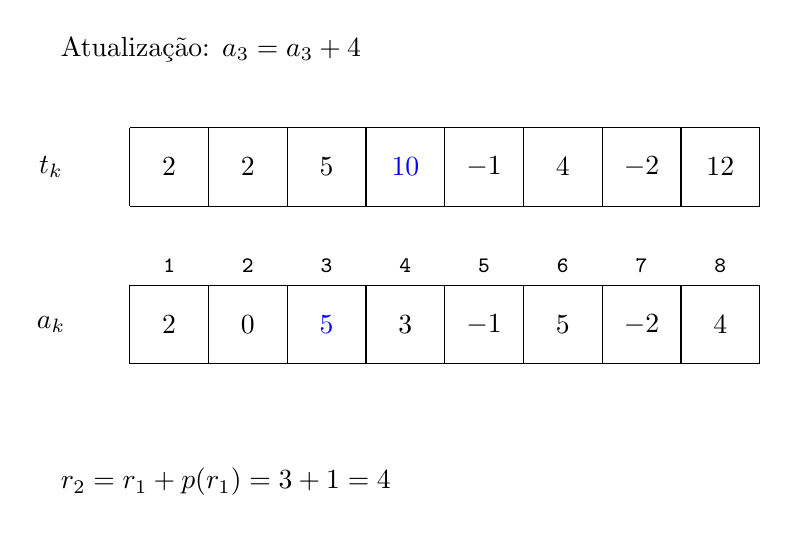
\begin{tikzpicture}
            \node[anchor=west] at (0, 12) { Atualização: $a_3 = a_3 + 4$ };

            \draw (1, 10) grid (9, 11);
            \draw (1, 8) grid (9, 9);

            \node at (0, 8.5) { $a_k$ };
            \node at (0, 10.5) { $t_k$ };

            \node[anchor=west] at (0, 6.5) { $r_2 = r_1 + p(r_1) = 3 + 1 = 4$ };

            \node at (1.5, 9.25) { \footnotesize \tt 1 };
            \node at (2.5, 9.25) { \footnotesize \tt 2 };
            \node at (3.5, 9.25) { \footnotesize \tt 3 };
            \node at (4.5, 9.25) { \footnotesize \tt 4 };
            \node at (5.5, 9.25) { \footnotesize \tt 5 };
            \node at (6.5, 9.25) { \footnotesize \tt 6 };
            \node at (7.5, 9.25) { \footnotesize \tt 7 };
            \node at (8.5, 9.25) { \footnotesize \tt 8 };

            \node at (1.5, 8.5) { \textcolor{black}{$2$} };
            \node at (2.5, 8.5) { \textcolor{black}{$0$} };
            \node at (3.5, 8.5) { \textcolor{blue}{$5$} };
            \node at (4.5, 8.5) { \textcolor{black}{$3$} };
            \node at (5.5, 8.5) { \textcolor{black}{$-1$} };
            \node at (6.5, 8.5) { \textcolor{black}{$5$} };
            \node at (7.5, 8.5) { \textcolor{black}{$-2$} };
            \node at (8.5, 8.5) { \textcolor{black}{$4$} };

            \node at (1.5, 10.5) { \textcolor{black}{$2$} };
            \node at (2.5, 10.5) { \textcolor{black}{$2$} };
            \node at (3.5, 10.5) { \textcolor{black}{$5$} };
            \node at (4.5, 10.5) { \textcolor{blue}{$10$} };
            \node at (5.5, 10.5) { \textcolor{black}{$-1$} };
            \node at (6.5, 10.5) { \textcolor{black}{$4$} };
            \node at (7.5, 10.5) { \textcolor{black}{$-2$} };
            \node at (8.5, 10.5) { \textcolor{black}{$12$} };

        \end{tikzpicture}

    \end{figure}

\end{frame}

\begin{frame}[fragile]{Visualização de uma atualização em uma BITree}

    \begin{figure}
        \centering

        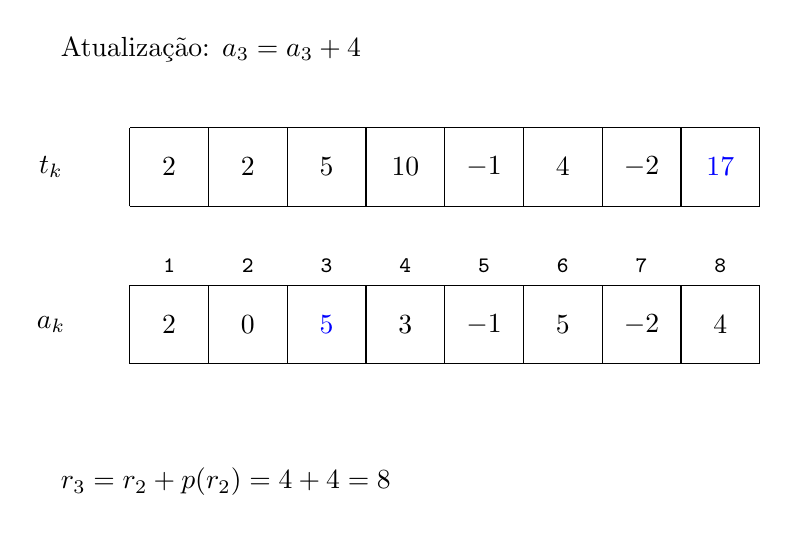
\begin{tikzpicture}
            \node[anchor=west] at (0, 12) { Atualização: $a_3 = a_3 + 4$ };

            \draw (1, 10) grid (9, 11);
            \draw (1, 8) grid (9, 9);

            \node at (0, 8.5) { $a_k$ };
            \node at (0, 10.5) { $t_k$ };

            \node[anchor=west] at (0, 6.5) { $r_3 = r_2 + p(r_2) = 4 + 4 = 8$ };

            \node at (1.5, 9.25) { \footnotesize \tt 1 };
            \node at (2.5, 9.25) { \footnotesize \tt 2 };
            \node at (3.5, 9.25) { \footnotesize \tt 3 };
            \node at (4.5, 9.25) { \footnotesize \tt 4 };
            \node at (5.5, 9.25) { \footnotesize \tt 5 };
            \node at (6.5, 9.25) { \footnotesize \tt 6 };
            \node at (7.5, 9.25) { \footnotesize \tt 7 };
            \node at (8.5, 9.25) { \footnotesize \tt 8 };

            \node at (1.5, 8.5) { \textcolor{black}{$2$} };
            \node at (2.5, 8.5) { \textcolor{black}{$0$} };
            \node at (3.5, 8.5) { \textcolor{blue}{$5$} };
            \node at (4.5, 8.5) { \textcolor{black}{$3$} };
            \node at (5.5, 8.5) { \textcolor{black}{$-1$} };
            \node at (6.5, 8.5) { \textcolor{black}{$5$} };
            \node at (7.5, 8.5) { \textcolor{black}{$-2$} };
            \node at (8.5, 8.5) { \textcolor{black}{$4$} };

            \node at (1.5, 10.5) { \textcolor{black}{$2$} };
            \node at (2.5, 10.5) { \textcolor{black}{$2$} };
            \node at (3.5, 10.5) { \textcolor{black}{$5$} };
            \node at (4.5, 10.5) { \textcolor{black}{$10$} };
            \node at (5.5, 10.5) { \textcolor{black}{$-1$} };
            \node at (6.5, 10.5) { \textcolor{black}{$4$} };
            \node at (7.5, 10.5) { \textcolor{black}{$-2$} };
            \node at (8.5, 10.5) { \textcolor{blue}{$17$} };

        \end{tikzpicture}

    \end{figure}

\end{frame}
